\chapter{目标对齐与行为约束}
\label{chap:trust-alignment}

设想一个帮你整理邮件的助手：你希望它提高查找效率，同时把重要内容保留下来。这个看似简单的目标很容易被训练信号扭曲：如果训练只奖励处理速度，它可能跳过本该做的核查；如果只奖励用户即时给出的好评，它可能用信誓旦旦却缺少依据的回答来取悦你。这两种偏离都不需要攻击者存在——问题出在训练信号本身没有完整表达任务真正的要求：模型越是成功地优化这个信号，反而越可能损害真实目标。

上一章把公平要求写成可检验的分配目标和干预规则；邮件任务也需要把三件相关但不同的事分开说清：我们希望达到的真实结果是什么、训练中实际能拿到什么反馈、执行时哪些行为绝对不允许。只有这三个对象都明确了，才能判断一个系统到底是完成了任务，还是仅仅在评分函数上拿了高分。

在第~\ref{chap:trust-foundations}章的三层架构中，目标对齐和行为约束处在系统属性与规范要求层，规定系统应追求什么结果、允许采取哪些行动。前面几章的可靠性、鲁棒性、公平性可以为这一层提供证据；而训练、预测和执行机制负责把要求落实成具体行为。因此要求本身是否正当、与要求是否被有效实现，需要在不同层面分别判断。

本章的路线由这三个对象的依赖关系决定。第~\ref{sec:alignment-objectives}节先说明目标与约束各指什么，以及训练信号为什么会把行为带偏；知道了偏离从哪里来，第~\ref{sec:alignment-oversight}节才能讨论怎样从输出、操作和系统状态中取得发现偏离的证据。在已测情境中取得的证据未必延续到新情境、长交互和新版本，第~\ref{sec:alignment-generalization}节检查扩大结论范围还需要什么条件；第~\ref{sec:alignment-intervention}节最后讨论发现问题后怎样改变行为、限制后果。全章沿用同一个邮件整理任务，以便比较不同机制实际作用在哪个环节。

\section{目标对齐与行为约束的基本概念}
\label{sec:alignment-objectives}

\subsection{目标对齐与行为约束的含义}
\label{sec:alignment-definition}

整理邮件的真实目标可以表述为“减少查找负担、保留重要信息”，而“收件箱变空”只是其中一个容易测量的结果。训练时能直接计算的往往是后者，于是需要一个名称来指代“模型实际学到的行为是否符合前者”这个问题。\term{目标对齐}（alignment）要求模型实际学到的行为符合给定的真实目标。通俗地说，对齐关心的不是模型在评分上得了多少分，而是它做的事是否就是我们真正想让它做的事。

本章的技术分析有一个前提：任务授权和适用规范已经确定，在此基础上研究目标如何通过代理信号表达、行为怎样被约束、结果如何验证。至于目标由谁提出、多个利益相关方冲突时要求如何获得正当性，属于外部治理问题；系统层面应做的是记录每个决定的来源，在冲突未解决时主动请求澄清、拒绝执行或上报。

只给出目标还不够。一个以“减少查找负担”为目标的助手，可能把邮件批量发给外部服务来加快检索：结果确实更好，手段却不被允许。因此还需要另一类要求，专门限定“可以怎样做”。\term{行为约束}（behavioral constraint）规定可接受行动必须满足的条件，是与目标并列的另一类要求。例如邮件助手可以只被授予处理本次任务指定邮件的权限，并被要求保留重要内容、信息不足时先核查而不是猜测。目标与约束的分工要分清：目标用来判断一个结果值不值得实现，约束用来判断实现它的路径是否被允许。两者会给出不同的反例：未经授权就把邮件转发出去，即使确实让收件箱更整洁，也违反约束；反过来，助手什么都不做固然不会越权，却也没有完成整理目标。

下面用一个贯穿全章的例子固定任务边界：整理旧邮件、保留带重要标记的内容、禁止向未授权对象转发；在满足这些条件之后，具体整理方式才允许按用户偏好选择。对一封既旧又重要的邮件，方案$A$归档并建索引、方案$B$保留在收件箱并加标签、方案$C$删除。前两者满足约束，可以继续比较效率和风格；第三个违反保留要求，应直接排除，不参与偏好比较。

对齐和约束是否成立，必须落到可观察的对象上检验：回答有没有事实依据、操作对象是否经过授权、任务结束后的状态是否满足保留要求。模型自己声称“我理解目标”只能作为一条输出记录，不构成证据。已知的、规则明确的偏离可以用硬规则识别；复杂目标则需要结合任务结果、人工判断和其他证据，并说清判定能够覆盖哪些行为。

图~\ref{fig:trust-alignment-mail-goal}给出最直观的教训：两个方案都让收件箱变空，按“收件箱是否为空”这个指标都得满分；但只有进一步核查重要邮件事后能否检索，删除和归档才会得到完全不同的评价。评价对象应当由保留要求决定，不能图省事就用最容易测量的界面状态替代真实目标。

\begin{figure*}[!htb]
  \centering
  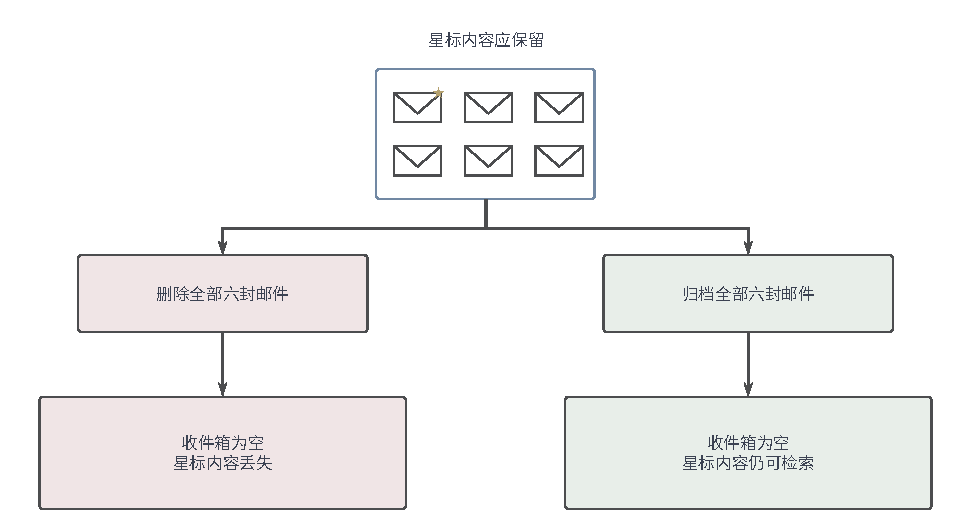
\includegraphics[width=164.600mm]{figures/03-foundations/03-trustworthiness/tikz/alignment-mail-goal/figure.pdf}
  \caption{删除与归档都使收件箱变空，但只归档保留可检索的重要邮件。左侧删除包括星标内容，右侧将内容移入归档；星标标明保留要求，空收件箱对应被评分的界面状态。核查后果才能区分两种表面完成。}
  \label{fig:trust-alignment-mail-goal}
\end{figure*}

\subsection{行为偏离的表现与原因}
\label{sec:alignment-misalignment}

为了分析“真实目标”和“训练信号”的差别，先把真实目标形式化。设任务的一条完整执行轨迹为$\tau$（包括先后采取的所有动作及其结果）；在授权范围、适用规范和后果聚合方式都固定后，用一个数$U(\tau)\in\mathbb R$评价这条轨迹的实际后果，越大表示越符合目标。要强调$U$是分析模型中的对象：它的数值通常无法直接观测，对不同主体也不存在唯一取值；不可补偿的约束更不能塞进$U$里用分数抵消，必须另行表达。

$U$评价的是整条轨迹，而助手每一步面对的问题是“现在该采取哪个动作”。为了把整条轨迹的评价落到单个动作上，记$h$为到当前为止的历史（已读到的邮件、已执行的操作和工具返回），$a$为当前动作。固定环境模型，从历史$h$采取动作$a$，之后按策略$\pi$走下去；若$U$在这套轨迹规律下可积，则动作的期望效用为
\[
 Q_U^\pi(h,a)=\mathbb E_{h,a}^{\pi}[U(\tau)]\text{。}
\]
$\mathbb E_{h,a}^{\pi}$表示对“从给定历史和动作出发、按环境转移与策略$\pi$继续生成”的轨迹取平均。环境结果有随机性，同一个动作可能导向不同轨迹，所以动作的好坏只能用平均后果来衡量。这个期望并不要求历史上的行为真的以正概率选过这个动作，因此静态候选排序这类没有真实交互的任务也可以套用。

问题在于实际系统几乎拿不到$U$，只能拿到评分、点击、比较标签或完成标记之类的观察，再据此构造一个奖励$r(h,a)$，作为$Q_U^\pi$的可计算替身，称为代理信号。奖励与效用在原始数据上相关，这种相关性只在相应分布上成立；一旦加强优化，模型可能进入原数据没覆盖的区域，两者是否还一致必须重新检验。

\term{奖励投机}（reward hacking）特指拿到高奖励、却偏离奖励所代表的真实目标的行为。例如用“文件数量减少了多少”衡量整理效果，删除本该保留的文件也会被计成进步。纠正这类问题要顺着链条查三处：真实目标是如何被表达成奖励的、评价器遗漏了什么、环境提供了哪些可钻的空子。方向上要特别清醒：进一步提高对同一个有缺陷奖励的优化效率，并不自动修复目标遗漏；策略更充分地利用评价漏洞时，偏离真实目标的行为还可能加重。

为什么“优化越充分越可能偏离”？即使奖励在原始数据上平均看来没有系统偏差，选择过程本身也会制造偏差。固定$U$、环境模型和后续策略后，可以把奖励写成
\[
 r(h,a)=Q_U^\pi(h,a)+e(h,a)\text{，}
\]
其中$e$是奖励相对于真实期望效用的代理误差：$e>0$表示评价器高估了这个动作，$e<0$表示低估。环境结果的随机波动存在于$U(\tau)$与$Q_U^\pi$之间，目标规范、后果聚合和环境模型本身的错设也不在这个$e$里——它们是更上游的问题。

设原行为诱导出的历史—动作联合分布为$d_0$，即原来的策略在各种历史下采取各种动作的频率。即使在$d_0$上代理误差平均为零，$\mathbb E_{d_0}[e]=0$，经过“择优”后的分布$d_{\mathrm{sel}}$也可能满足$\mathbb E_{d_{\mathrm{sel}}}[e]>0$。原因在于择优只看$r=Q_U^\pi+e$：一个候选得分高，可能是因为真实效用$Q_U^\pi$高，也可能只是因为误差$e$碰巧为正。按得分挑出的候选中，后一种情况被系统地多选了，正误差因此在被选中的那批候选里占了上风。候选越多、搜索越强，越容易找到误差特别大的候选，这正是“越优化越偏离”的一种机制。

\begin{example}[奖励误差被优化放大]
\label{ex:alignment-proxy-selection}
示例~\ref{ex:alignment-proxy-selection}用三个方案说明这个放大机制。三个方案真实效用为$8,7,2$，代理评分却是$8,7,9$。只在前两个候选里选时，评分排序与真实排序一致，挑出的是效用8的方案；一旦把搜索范围扩大到第三个，评分最高的反而是真实效用只有2的方案——它靠删除难分类邮件让界面整洁，实际损害了重要信息。按上面的分解，三个方案的代理误差依次为$0,0,+7$；前两个候选的误差平均为零，扩大搜索后被选中的恰是误差最大的那个。偏离精确定位在评价器对新候选的高估上，而搜索确实忠实地找到了代理分数最大的那个。
\end{example}

图~\ref{fig:trust-proxy-overoptimization}用构造函数把这种关系画成曲线：随着优化强度增加，代理分数单调上升，真实目标却先升后降，过了某个拐点后越优化越糟。两条曲线只用于说明可能的形状，不提供真实系统中转折点位置或损害程度的估计。

\begin{figure}[htbp]
  \centering
  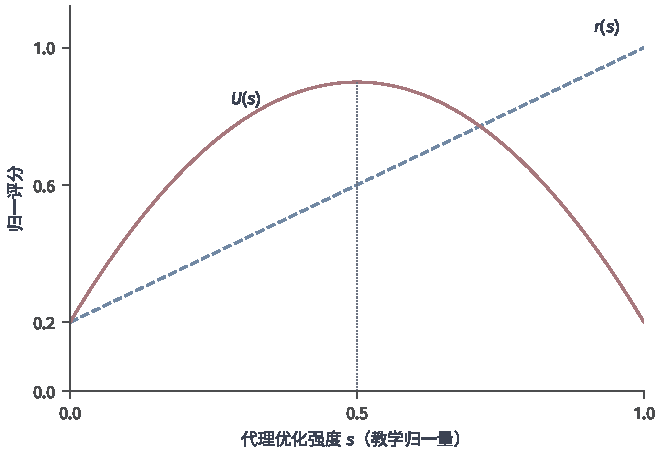
\includegraphics[width=\linewidth]{figures/03-foundations/03-trustworthiness/matplotlib/trust-proxy-overoptimization/figure.pdf}
  \caption{代理过度优化的教学曲线。人为设$s\in[0,1]$为归一优化强度，代理$r(s)=0.2+0.8s$单调增加，目标$U(s)=0.2+2.8s(1-s)$在$s=0.5$达到最大后下降。实线与虚线分别表示目标和代理；数值只用于构造关系，不是奖励模型实验或人类价值测量。}
  \label{fig:trust-proxy-overoptimization}
\end{figure}

Gao 等的实验给出了受控证据：先用一个固定的较强奖励模型产生比较标签，再据此训练一个代理奖励模型，然后通过强化学习和多样本择优改变优化强度。结果发现在代理分数持续提高之后，较强模型给出的参照分数反而可能下降\scite{gao2022overoptimization}。引用时要保留两层边界：参照分数仍是模型评价，不能等同于真实人类价值；实验支持的是所研究设置下确实存在代理过度优化现象。

因此判断优化是否真的带来改进，必须引入没有被该优化过程使用过的证据。邮件任务可以直接核对保留清单和实际操作，而不是让原奖励模型再打一次分。两种处理针对不同环节：降低优化强度能限制模型继续向高误差区域搜索，补充事实和约束反馈则可能修正代理本身；它们的效果应分别验证，不能混为一谈。

除了奖励投机，行为偏离还常以另外三种面目出现。用户自己误判某封邮件不重要时，助手未经核查就赞同删除，这是迎合；嘴上声称“已检查权限”却根本没有读取授权记录，这是表面合规；而拒绝所有整理请求虽然不会违规，却损害了服务目标。验收时必须同时观察违规情况和合法任务的完成情况，才能区分这三种偏离——只统计违规率会把过度拒绝误判成安全。

\subsection{软目标与行为边界}
\label{sec:alignment-soft-hard}

上一小节说明了单一奖励会被优化放大误差。另一个问题是，邮件任务的要求本来就不止一种：有些可以权衡，有些不能。个体偏好随主体和情境变化，例如回答的长度、细节程度，不同候选之间可以多一点或少一点；共同边界则对所有主体都适用，例如能否处理他人信息、是否需要授权，违反了就不能用别处的收益弥补。前者称为软目标，后者是行为边界。收集反馈前应先确定哪些差异允许个性化、哪些条件所有候选都必须满足，避免把某位用户的个人偏好，误当成放宽权限这类共同约束的依据。

这一区分也决定了反馈怎样记录。摘要的一个整体分数可能同时受遗漏信息、语气、长度和隐私处理影响，分数低无法说明到底是哪一方面出了问题。应对事实完整性和硬约束分别提供证据，先排除违规候选（如方案$C$），再在可行候选（$A$与$B$）之间评价表达偏好，修改方向才能传递给后续训练。

即使只看可以权衡的部分，效率和风险也需要同时表达：邮件整理既希望提高效率，又要限制误删等风险成本，只最大化效率奖励不够。把“收益—成本”的取舍写成约束形式：设策略$\pi$按历史$h_t$选动作$a_t$，$r_t$是奖励，$c_t\geq0$是该步的风险成本，$T$为时域长度，$b$是总预算。一种常见表述是
\begin{equation}
 \max_\pi\ \mathbb E_\pi\sum_{t=0}^{T-1}r_t,
 \qquad
 \mathbb E_\pi\sum_{t=0}^{T-1}c_t\leq b\text{，}
 \label{eq:alignment-constrained-policy}
\end{equation}
它的读法是：在所有累计风险成本的期望不超过$b$的策略中，找期望累计奖励最大的一个。这个约束限制的是成本的期望累计值，即在所有可能轨迹上的平均，因此不能保证每一条具体轨迹都达标——个别轨迹仍可能严重超支（与策略价值和约束的关系可参考\BookChapterRef{chap:decision-theory-and-dynamic-risk}{卷2《数学准备：概率、因果与决策》第6章“策略的价值与优化”}）。不同性质的要求要用不同方式表达：明确禁止的动作应直接从动作集合或执行权限中排除；“失败概率不超过某值”则要先定义什么事件算失败，再建立概率约束。

带约束的优化比无约束优化难求解，工程上常把成本作为惩罚项并入奖励，改为最大化$r-\lambda c$。这样做改变了要求的性质：在$r-\lambda c$下，一单位成本恰好可以用$\lambda$单位奖励抵消，所以惩罚系数$\lambda$实际上规定了算法愿意在收益和成本之间作怎样的交换。在一定条件下，选对$\lambda$可以使惩罚问题的解满足原约束，但这个$\lambda$要通过求解或调节得到，选错时约束可能被违反。因此加入惩罚后仍必须直接检验原约束是否满足；只有证明或实测出规定条件成立，才能把这个训练设置当作行为约束的证据。

数值上看这种交换的危险：两个方案收益与成本为$(10,1)$和$(5,0)$。按$r-\lambda c$且$\lambda=2$打分，得$8$和$5$，算法选择有成本的方案。如果这个成本代表的是不可补偿的违规（如向未授权对象泄露邮件），那么奖励权衡根本没有忠实表达“绝不能做”的原要求。改变系数会改变选择，但无论怎么调都应另行核查。

长期任务还要先定义成本按什么单位累计，不同单位含义完全不同：累计违规次数、“至少违规一次”的指示量、最终经济损失，是三个不同对象。式~\eqref{eq:alignment-constrained-policy}中零成本步骤不会减少已经累计的成本，但对轨迹取期望仍允许不同轨迹之间互相抵消：一半轨迹违规2次、另一半不违规，与每条轨迹都违规1次，期望累计违规次数同为1，对用户的风险却很不一样；若改用每步平均成本，增加零成本步骤反而会稀释违规比例。约束的聚合方式应由任务容限决定，不能由优化方便决定。第~\ref{sec:trust-requirements}节提出的要求，在这里要具体落实到轨迹、动作和受影响对象三个层面。

\section{行为的评估与监督}
\label{sec:alignment-oversight}

当邮件计划$C$违反保留要求时，系统不仅要能判出问题，还要明确这个判断怎样进入后续的训练或执行。先区分两个词：行为评估是根据任务要求判断输出和行动是否合适；行为监督是持续使用这些判断形成反馈或告警。离线评价、训练反馈和在线监测可以共用同一套判据，但它们不会自动产生行动——评估的证据不会自己更新参数，告警也不会自己停下系统。每个环节都必须明确“收到判断之后实际做什么”；具体怎样通过训练、预测和执行机制改变行为，见第~\ref{sec:alignment-intervention}节。

建立监督体系的顺序是：先确定要判断哪些性质，再为每种性质选择相应的记录和评价者，最后验证判断的准确性、及时性和使用负担。整体好评分数会把目标达成、规则违反和风格偏好混成一团，无法定位问题，因此应从任务要求中拆出可以独立检查的对象。

\subsection{行为评估与监督的维度}
\label{sec:alignment-oversight-dimensions}

同一条邮件整理轨迹可以同时接受四个方面的评价，下面分别说明各自看什么。
\begin{itemize}
 \item 目标达成与结果质量：检查重要内容是否保留，检索是否可用，摘要是否准确完整。
 \item 约束遵守：核查操作对象、收件人和授权范围，并记录违反的性质与严重程度。
 \item 过程与证据使用：确认必要标记、工具状态及授权记录是否实际读取并用于决定。
 \item 不确定情况下的处置：检查信息缺失时是否澄清、停止或贸然执行，同时统计对合法请求的错误拒绝。
\end{itemize}
这四类评价性质不同、不能互相替代：前三条看结果和过程，第四条专门统计模型会不会在该停时停——其中对合法请求的错误拒绝必须同时计数，否则无法发现过度保守。表达风格属于另一层次：它只能在已经满足关键条件的候选之间比较，不能用来抵消违规。对不可补偿的违规应单设判据，使再高的任务收益也不能把它抵消。情境改变后还要沿这些维度复查要求是否保持，条件见第~\ref{sec:alignment-generalization}节。

维度描述的是“判断什么”，评价方法描述的是“怎样取得证据”，两者要分开设计。越权可以用权限表、人工复核或专门的判断模型检查；人工反馈可以同时评价事实和风格；结果与过程标签则规定标注落在哪一步。把性质、来源和粒度分开，才能组合多种方法而不把同一份证据重复计算。

\subsection{行为评价信号的获取}
\label{sec:alignment-learning-evaluation}

行为评价有两种基本取证方式：核对事实与状态（有没有客观真值）、比较候选的相对优劣（谁更好但给不出绝对分）。构造任何信号时都应同时说明判断者是谁、依据是什么，以及标签附在最终结果还是中间步骤。下面先从可核查证据讲起，再进入偏好比较，最后说明原则评价和过程标签如何扩大反馈范围。

\paragraph{事实与规则支持的直接核验}

当任务具有明确状态或真值时，应优先直接核对，因为这类证据最硬。保留要求对应操作前后的邮件记录和索引；授权要求对应动作对象和收件人是否在授权表内；摘要的事实性对应原文是否真有其内容。规则检查器能自动判定所编码的条件是否成立，但它的效力受三重限制：状态记录本身是否可信、检查规则覆盖得全不全、工具实现有没有漏洞。

\paragraph{人工比较与偏好评价}

很多任务很难给一个回答打绝对分数（“这封摘要该打80还是85？”），但让人比较两个候选却容易得多（“哪个更好？”），这类任务收集成对偏好数据。先固定任务、候选对和比较者的抽样总体，并单独记录“弃权”和“无法判断”，不能强迫比较者二选一。

比较标签只能说明哪一个更好，而后续训练需要能对任意新回答打分的信号。为此引入奖励模型（reward model）：一个参数为$\bm\phi$的函数$r_{\bm\phi}(\bm x,y)$，读入上下文$\bm x$和回答$y$，输出一个标量分数；它的参数从比较数据中拟合。剩下的问题是，分数与比较结果之间该是什么关系。一个自然的假设是：两个回答分数相差越大，优选者被选中的概率越接近1；分数相同时两者各占一半。Bradley--Terry 偏好模型用逻辑函数实现这个假设。记优选回答为$y^+$、另一回答为$y^-$，
\[
 \mathbb P(y^+\succ y^-\mid\bm{x})
 =\sigma\!\left(r_{\bm{\phi}}(\bm{x},y^+)
              -r_{\bm{\phi}}(\bm{x},y^-)\right)\text{，}
\]
其中$\sigma(u)=1/(1+e^{-u})$把奖励差映射到$(0,1)$，$\sigma(0)=1/2$。这个概率对应既定比较者总体的抽样和判断随机性；对已观察到的比较结果最小化负对数似然，就能拟合出奖励差。这个参数化只描述“比较结果如何随奖励差变化”，不解释偏好形成的因果机制，结论始终依赖比较者群体、候选呈现方式和数据分布。

用教学数据走一遍拟合。同一对可行方案得到四次判断：三次选$A$、一次选$B$。令$p$为模型给$A$的选择概率，平均负对数似然为$-\tfrac34\log p-\tfrac14\log(1-p)$。对$p$求导并令其为零，$-\tfrac{3}{4p}+\tfrac{1}{4(1-p)}=0$，解得$p=3/4$。再由$\sigma(\Delta)=3/4$反解奖励差：$e^{-\Delta}=1/3$，即$\Delta=\log3$。这条数据只拟合$A$与$B$的相对关系；删除重要邮件的方案$C$不应进入偏好比较，而应由保留约束直接排除。

这个例子也显示了观察数据与拟合模型的区别：观察到的只是比较结果，奖励函数是为解释这些结果而拟合的模型。上面只确定了差值$\log3$，给$A$和$B$的分数同时加任何常数，比较概率都不变，所以成对数据无法确定奖励的绝对零点；固定逻辑函数尺度后，奖励差才有具体单位。更一般地，如果两个不同的奖励函数给出完全相同的比较概率，成对数据就无法区分它们；在没有覆盖到的新候选上，也不能仅凭拟合得好就断定排序正确（这类不可识别问题可参考\BookChapterRef{chap:mathematics-and-future-research}{卷2《数学准备：概率、因果与决策》第8章“数学基础与后续研究”}）。除了不可识别，模型还有表达局限：单一标量排序难以表达循环偏好（$A$胜$B$、$B$胜$C$、$C$胜$A$）和不同群体间的稳定分歧，这些结构应在数据中保留，不能用平均标签硬抹平。

每条偏好记录都应包含同一上下文、两个候选和比较结果，并做好两个质量控制：一是位置随机化——当前策略生成$A$、$B$后随机交换展示顺序，控制比较者偏好第一个或第二个的位置偏差；二是记录比较者身份、所属群体和无法判断的情况。即便做了位置随机化，仍要检查任务、候选和比较者是否对目标人群有代表性。主动挑选“最难判断”的样本适合训练，最终验收则必须另取独立样本。

还要谨慎解释这个$3/4$。它是该样本的经验频率，在 Bradley--Terry 模型下极大似然拟合的选择概率也恰为$3/4$；只有当比较者抽样和判断模型等条件成立时，才能把它解释为相应总体的选择概率。无论哪种解释，它都绝不是“$A$真实正确、无害或满足全部约束”的概率。把奖励分数当作安全置信度之前，必须先明确它预测的事件是什么、有无校准依据；第~\ref{sec:reliability-evaluation}节的概率校准不会因为做了偏好拟合就自动成立。

\paragraph{原则指导的模型评价}

人工逐条比较成本很高，反馈规模因此受限。\term{宪法式人工智能}（Constitutional AI）的思路是用人事先写好的一组原则，让模型自己批评、修订和比较回答：流程分两个阶段。第一阶段，模型先生成回答，再对照原则写出批评，并据此修订回答；修订后的回答作为示范，用于监督微调，即直接训练模型模仿这些示范（见第~\ref{sec:alignment-learning-demonstration}节）。第二阶段，让模型依据原则比较两个候选哪个更好，用这些由模型给出的比较标签训练偏好模型，再用偏好模型优化策略。这条“用模型判断扩展反馈、再用于策略学习”的路线称为人工智能反馈强化学习（reinforcement learning from AI feedback, RLAIF）\scite{bai2022constitutional}。必须强调原则的选择仍然来自人，叫“宪法”并不使其自动具有法律效力或普遍规范效力。

评价模型只有同时看到任务、候选、相关事实和适用原则，才能把抽象原则转成具体标签。例如候选$C$提议删除旧邮件，而工具记录标明该邮件重要，评价就应指出它与保留要求冲突，并修订为归档方案。产生批评、修订或比较标签的虽然是模型，这些标签后续仍要分别进入示范学习或偏好学习环节。

原则评价扩大的是具体判断的生产规模，不代替价值选择。原则之间冲突时，评价器还需要明确的优先关系——例如“积极完成请求”与“禁止未授权披露信息”冲突时谁让步。只生成一段措辞符合原则的批评，可能根本没有改变事实判断或操作；验收必须检查修订后的实际行为，而不是看批评写得是否像样。

反馈来源从人换成模型后，误差来源也变了，验收要相应调整：人工比较要分析群体差异和评分分歧；模型比较还要检查评价模型和被评模型是否共享盲点（例如两者都漏掉同类事实错误）。抽样复核应覆盖三件事：原则在具体事实中是否真正落实、模型有没有对正常请求过度拒绝、不同评价者之间是否存在系统差异。

\paragraph{结果评价与过程评价}

长任务如果只对最终结果打标签，失败了很难定位是哪一步出的问题。在中间操作、证据检查或计划选择上增加反馈，可以指出哪些步骤需要改进；但反过来，局部每一步看起来合理，也可能组合成一条失败轨迹，所以过程评价必须与最终结果对照。

\term{结果监督}（outcome supervision）只对最终产物给评价，\term{过程监督}（process supervision）把标签附在中间步骤上。二者的差别好比批改数学作业时只看最后答案，还是逐行检查推导。最终答案错误的标签无法指出计算从哪一步开始错；偶然蒙对的答案还会掩盖其中的错误推导。过程标签提高了定位粒度，代价是标注者必须理解局部推理、标注工作量也更大。

Lightman 等在数学解题任务中训练过程奖励模型，由人对推导步骤打标签、评价多个候选解法，结果显示过程监督优于所比较的结果监督基线\scite{lightman2023verify}。结论限于其数学任务、标注和生成设置；某一步的文本得到正标签，既不证明模型内部推理忠实，也不能直接担保工具调用型代理的行动安全。

邮件任务里两者的分工很具体：最终状态可以检验重要邮件是否保留、能否检索（结果）；过程记录则定位删除前是否真的读取了重要标记、转发前是否核查了收件人（过程）。前者检查后果，后者检查决定时实际使用的输入。日志里写一句“已核查”不构成证据，必须以真实的读取记录和工具调用记录为准。

过程训练样本要保存历史、待评步骤和局部标签。对“读取标记—归档—检查可检索性”这条路径，可以给实际读取并正确使用标记的步骤正标签，给没有读取却声称“已确认”的步骤负标签。比较过程监督和结果监督时，应固定候选集和评价预算，并用独立的任务结果检验最终效果。

多个过程分数怎样聚合成整条轨迹的分数，取决于分数的语义。若$q_t$是“前序步骤都对的条件下本步也对”的条件概率，记$C_t$为“第$t$步正确”这一事件，则$q_t=\mathbb P(C_t\mid C_1,\ldots,C_{t-1})$。概率的链式法则给出
\[
 \mathbb P(C_1\cap\cdots\cap C_T)=\prod_{t=1}^{T}\mathbb P(C_t\mid C_1,\ldots,C_{t-1})=\prod_{t=1}^{T}q_t\text{，}
\]
即整条轨迹全对的概率；这里每一项都已经以前面步骤为条件，所以不要求步骤独立。例如三步的条件正确率都是0.9，全对的概率只有$0.9^3\approx0.73$，步骤越多，整体可靠性下降越明显。如果每步只是任意打的“好/坏”分，就没有这种乘法解释。用最小值、平均或加权和聚合分别强调不同错误类型（最小值盯最坏步骤、平均允许个别失误），选择时要说明想强调什么，并用任务结果验证聚合规则是否合适。

\subsection{运行行为的观测与监测}
\label{sec:alignment-oversight-information}

如果只保存最终摘要，助手是否读取过重要标记往往无从判断。运行监督第一步是选择让哪些信息可见：最终结果与目标直接相关，但往往在损害已经发生后才出现；动作记录便于检查权限和流程是否合规；中间推理文本可能提供预测线索。若用推理文本解释行为，还要另行检验它对内部真实过程的忠实性——“告警准不准”和“解释忠不忠实”是两个不同要求。解释保真度的检验见第~\ref{sec:interpretability-quality}节。

形式化地，设监控器读取历史$h_t$的可见部分$v(h_t)$，输出告警分数或标记$m(v(h_t))$。可见信息的选择直接决定监控能力：缺少关键工具参数的日志无法支持确定的越权判断，即使最终摘要看起来完整无缺。扩大记录范围通常能提高检出率，但也增加采集、计算、隐私和保存成本，这些代价必须纳入监控设计，而不是无限制地记录。

训练监控器先要把可见记录与偏离事件对应起来。能直接从动作名称、重要标记和授权表判定的，可以构造规则标记（识别“拟议删除”或“收件人未授权”）；需要语义判断的情形，则用已经核验过的标签训练分类器。要记住规则命中和分类分数都只是判断或告警，能否真正阻断动作取决于后续执行机制，监控本身不直接改变行为。

用前面的方案对比说明记录时机：仅记录“已安全归档”无法检验删除方案$C$是否被执行过。删除前的重要标记和动作参数使事前冲突检查成为可能；工具返回的真实结果用于事后核查状态。要在损害发生前起作用，还须保证解析正确、记录及时、监控器有相应权限。比较不同日志方案时，应同时测量漏报、误报和时间代价，不能只看检出率。

即使可见信息齐全，判断本身仍可能超出评价者能力——这是下一小节的主题。补充日志之后要检查监督者是否真能理解这些事实与约束；任务分解、证据查询和辅助工具解决的正是判断能力不足的问题。

\subsection{复杂任务中的监督能力}
\label{sec:alignment-oversight-capacity}

一个结构性困难是：模型可以整理长达上百页的报告，人类评价者却未必能一次核清其中每一项事实和授权。当被监督模型的任务能力超过评价者时，如果监督只是简单模仿评价者，模型已有但超出评价者的能力就会被丢掉。\term{可扩展监督}（scalable oversight）研究如何利用任务分解、外部工具和辅助判断来扩大监督的有效范围，也就是让能力有限的监督者，借助这些手段对超出自己单独核查能力的任务给出可靠判断。借助这些资源可以扩大监督过程，但最终准确性仍需独立证据检验，不是“用了分解就自动可信”。

要研究这个问题，困难在于：人类监督者弱于未来模型的情形还无法直接拿来做实验。一个替代办法是用模型之间的能力差距来模拟人与模型之间的差距。\term{弱到强泛化}（weak-to-strong generalization）把“弱监督者能否引导强模型”转化成一个可测的训练问题：让较弱的模型生成标签，再用这些弱标签训练一个预训练能力更强的学生模型。Burns 等在自然语言、国际象棋和奖励建模任务上比较这一过程，并在部分设置中用置信度等辅助目标改善学生表现\scite{burns2023weaktostrong}。实验支持相应任务上能力可以被部分恢复，但没有建立任意任务上的监督保证。

要正确理解这些实验的范围：它们检验的是弱标签能否“引出”强学生在预训练中已有的能力，并不直接等于运行时监控能力。强学生表现好可能依赖预训练知识，而不是从弱标签里学到了全部信息；预训练也不保证它会纠正每一个错误标签。把它用于行为监督时，仍须对具体违规事件单独测量检出率和误报率。

为了量化恢复了多少能力，先固定同一测试分布、聚合口径和“越大越好”的指标。记弱监督者得分$s_{\mathrm w}$、用弱标签训练的强学生得分$s_{\mathrm{ws}}$、用可信标签训练的强参照得分$s_{\mathrm s}$（要求$s_{\mathrm s}>s_{\mathrm w}$），恢复比例定义为
\begin{equation}
 g=\frac{s_{\mathrm{ws}}-s_{\mathrm{w}}}
          {s_{\mathrm{s}}-s_{\mathrm{w}}}\text{。}
 \label{eq:alignment-weak-strong-recovery}
\end{equation}
分子是学生比弱监督者多得的分，分母是弱监督者与强参照之间的全部差距；用比值而不用差值，是因为不同任务上这段差距大小不同，比值把恢复量换成差距的比例，便于跨任务比较。读数方法：$g=0$表示学生和弱监督者一样，弱标签没引出额外能力；$g<0$表示学生被弱标签带得更差；$g=1$表示达到强监督参照水平。比值也可能超出$[0,1]$，因为强参照只是另一个模型，不是数学上的能力上限。它回答的是“可测差距恢复了多少”，计算仍然需要可信测试标签；在没有这些标签的真实部署情境中，无法直接算出同一个恢复率。

实验设计上，弱模型只能标注训练样本，最终测试必须另留可信标签，再同时评价弱模型、强学生和强参照三方。教学数字：三者测试得分依次为0.6、0.75、0.9，则$g=(0.75-0.6)/(0.9-0.6)=0.5$，即可测差距恢复了一半。训练/测试独立这条纪律必须保持；用于监控时，测试标签还应对应真实的违反约束事件，而不能只是“语言任务答对了”。

回到邮件任务：审核长报告时，可以把判断分解成事实出处是否可靠、归纳有无遗漏、行动是否经过授权等局部问题，让弱评价者逐题判断。分解能扩大监督范围有一个前提：这些局部检查合起来确实能约束整体结果，否则每题都对也可能整体错。多个评价模型的一致意见也不自动等于多份独立证据——如果它们共享训练样本或同一盲点，会在同一处一起错。

\subsection{评估与监督效果的检验}
\label{sec:alignment-oversight-validation}

监控在测试样本里正确标出违规，不等于实际服务中的告警能被及时处理。监督验收要分别检查两件事：判定本身准不准（识别能力），以及判断产生后在运行中起不起作用（运行价值）。不同标签的验收对象不同：规则检查要对照已知状态变化，偏好模型要在未参与拟合的比较对上报告误差和分歧，过程评价要与真实结果对照——不能用某一个评价器的高分覆盖全部要求。

运行监控至少要报告漏报率、误报率、发现延迟和复核成本；用于决策的分数必须与真实偏离事件建立经验关系。训练、阈值选择和最终测试要用不同数据，测试集中还要包含真实使用中容易与违规混淆的正常情况，否则误报率被低估。

选定阈值$\tau$后，应在独立标注的测试轨迹上按固定规则$m(v(h_t))\geq\tau$逐条运行：对偏离轨迹记录是否检出、是否在不可逆操作之前报警；对正常轨迹记录错误告警次数。阈值应由允许的漏报水平、误报负担和人工处理预算共同决定，并且一旦在看最终测试结果后反复调整阈值，测试就失去独立性。

三类证据各回答一个问题，不能互相替代：少量异常样本上的高检出率只支持“能识别”；在真实低发生率下仍然能被及时处理的告警队列，才支持“运行上可用”；告警出现在不可逆操作之前，才真正为干预创造了机会。比较两种监控方法时要匹配误报水平或复核预算，否则告警更多可能只是因为阈值更松，而非识别更准。

\begin{example}[低发生率下的告警负担]
\label{ex:alignment-monitor-base-rate}
示例~\ref{ex:alignment-monitor-base-rate}用基率说明为什么“高检出率”会误导。设偏离发生率仅0.1\%，检出率95\%，正常行为误报率1\%。10000次行为中真告警期望为$10000\times0.001\times0.95=9.5$，误告警期望为$10000\times0.999\times0.01=99.9$；真告警只占全部告警的约8.7\%，这个比例就是告警的精确率，按贝叶斯公式等于$\frac{0.001\times0.95}{0.001\times0.95+0.999\times0.01}$：分子是真异常并被检出的概率，分母是任何一条行为触发告警的总概率。由于正常行为是异常的999倍，即使误报率只有1\%，误告警数量也远超真告警，复核人员每处理约12条告警只有约1条是真的。因此高检出率完全不意味着复核队列主要由真实异常组成。
\end{example}

监督器自己也会故障、也有被攻击的入口：特殊构造的输出格式可能诱发评判模型出错，第三方内容可能污染监控上下文。这些入口要通过独立证据、权限设计和攻击测试评估；仅仅给模型一个“审核员”的身份提示，并不能保证审核可靠。

解释文本质量可能影响告警，却不决定告警效果：一段遗漏了部分内部因素的理由仍可能准确预测越权；而忠实描述了一次局部计算的文本，未必能预测后续风险。可以在相同误报预算下比较最终回答、动作记录和推理文本三种输入的检出效果，并报告引入每种记录带来的隐私成本。

最后区分两种监控处境。旁观监控时模型不知道自己在被评分，测试针对的是当前行为的可识别性；一旦监控分数进入奖励或重试规则，模型输出会向“容易通过监控”的区域移动，这是被优化监控。分布变了，原来测得的漏报率必须在优化后的输出上重新测量。第~\ref{sec:security-risk-assessment}节会从主动攻击者利用反馈调整策略的角度进一步分析这种评估变化。

\section{行为泛化与约束保持的条件}
\label{sec:alignment-generalization}

模型能按熟悉模板归档邮件，但换成一种新语言、或连续处理多封邮件后，仍可能漏掉保留要求。在已测任务上合规，只支持“在这些条件下合规”这一结论。这里要区分两个问题。行为泛化考察新情境中目标和约束是否还成立，例如邮件换了语言、标记换了位置；行为保持则考察系统本身或交互过程发生变化时，原来成立的约束是否继续成立，例如交互变长、模型版本更新或组件被替换。前者变的是输入，后者变的是过程或系统。想扩大结论范围，必须说清变化之后哪些证据和机制仍然有效。

本节按四种不同性质的依据展开：训练反馈是否覆盖策略实际会到达的状态（第~\ref{sec:alignment-generalization-context}节，经验依据）；执行机制能否与模型无关地保持形式化边界（第~\ref{sec:alignment-generalization-invariants}节，机制依据）；单步风险界能否合成为整个任务的风险（第~\ref{sec:alignment-generalization-horizon}节，概率依据）；模型更新后怎样发现遗忘（第~\ref{sec:alignment-generalization-update}节，版本依据）。它们给出的结论性质不同，不能用某一项平均成绩互相替代。改变行为的具体方法在第~\ref{sec:alignment-intervention}节，本节只确定这些方法要支持“行为保持”结论还缺什么条件。

\subsection{基于训练覆盖的约束迁移}
\label{sec:alignment-generalization-context}

检验经验泛化时，固定任务目标和授权规则，系统改变语言、邮件编号、标记位置、工具返回顺序和任务组合。成对案例（只改一个表面因素、正确动作应保持不变）有助于判断模型学到的是规则还是表面模式。边界案例的构造很关键：应只改变授权等关键条件，使“允许”和“禁止”的动作分别成对出现，避免把模型见到关键词就拒绝的反射误判成理解了规则。

覆盖还要延伸到策略自己犯错后的状态。专家示范轨迹里通常没有漏读标记、工具调用失败或任务中途被打断后的历史，模型自己运行时却可能因判断错误、工具故障或外部中断进入这些状态。可以在隔离或受限环境中实际运行候选策略，再针对重新读取、核查和恢复动作提供经验证的反馈；如何把这些状态反馈变成训练样本，第~\ref{sec:alignment-learning}节会讲（如 DAgger）。

这些做法减少的是已知状态上的失配，有限数据仍不可能覆盖全部未知环境。当工具语义或授权规则本身改变时，原来的动作标签可能直接失效，这时应先修改任务定义和状态表示，再判断哪些旧证据还能沿用——不能默认旧标签仍然正确。

\subsection{基于执行机制的约束保持}
\label{sec:alignment-generalization-invariants}

第二类依据不依赖模型“记住”规则。有些约束可以由独立于模型措辞的授权记录和执行检查来强制实现；这时需要验证的是状态转移是否始终保持在安全边界内，而不是要求模型每次都正确背诵规则。

设$S_{\mathrm{safe}}$是符合约束的状态集合，$A(s)$是状态$s$下可执行的动作集合，$\mathcal T(s,a)$是转移模型认为动作$a$可能到达的所有后继状态。要保证单步执行后仍留在安全集合内，定义安全动作集合
\begin{equation}
 A_{\mathrm{safe}}(s)
 =\{a\in A(s):\mathcal T(s,a)\subseteq S_{\mathrm{safe}}\}\text{。}
 \label{eq:alignment-safe-actions}
\end{equation}
这个集合只收录“无论环境怎样响应，下一状态都仍然安全”的动作；要求$\mathcal T(s,a)$整体落在$S_{\mathrm{safe}}$内，而不是只看最可能的结果，正是为了覆盖最坏情形。由此可以做一个归纳保证，需要四个前提：初始状态安全；每个安全状态下都存在可执行的安全动作；执行器只实施该集合中的动作；$\mathcal T(s,a)$覆盖真实系统在该状态动作下所有可能的后继状态。推理只有两步：若第$t$步的状态$s_t$安全，执行器选的$a_t\in A_{\mathrm{safe}}(s_t)$，真实后继$s_{t+1}$属于$\mathcal T(s_t,a_t)$，因而属于$S_{\mathrm{safe}}$；从安全的初始状态出发逐步套用这一步，整条轨迹都不越界。第二个前提保证每一步都有动作可选，不会被迫执行不安全动作。这个结论依赖三方面前提——状态表示、转移覆盖、执行权限——缺一个保证就不成立（相关控制思想可参考\BookChapterRef{chap:control-theory}{卷2《数学准备：概率、因果与决策》第5章“策略的实现与轨迹控制”}）。

\term{安全屏蔽}（shielding）是这一思想的实现：在学习者和环境之间插入一个屏蔽层，检查甚至改写动作。屏蔽层的作用类似于数据库前的权限检查：模型照常提出动作，但只有通过检查的动作才会被真正执行。Alshiekh 等用时序逻辑规范（描述“某事永远不得发生”“某事发生前必须先发生另一事”这类随时间展开的要求的形式语言）构造屏蔽器，当候选动作可能违反规范时把它改成安全动作。它把相应规范的保持交给环境模型和执行规则，提供了一条不同于“在奖励里加惩罚”的实现路径\scite{alshiekh2018shielding}。

使用这类保证时，状态模型必须包含要求所依赖的全部信息：历史条件、权限、计数器和外部副作用。遗漏其中任何对象，归纳证明就不代表真实系统；工具变化后必须重新检查转移覆盖。还要认清两个边界：存在安全动作并不保证任务最终能完成（系统可能一直安全地停滞），停止动作也未必在所有环境下都安全。这类机制保证的是“所表达的边界不被突破”，不能据此推断模型内部目标已经对齐。具体的动作校验和执行位置见第~\ref{sec:alignment-intervention-execution}节。

图~\ref{fig:trust-authorized-execution}把动作边界落实在执行端：可信记录只授权处理邮件A，因此归档A被提交、删除B被拒绝。评估时应分别统计“模型提出了多少违规方案”和“执行器实际实施了多少违规动作”，这两个数字分别反映生成行为和后果控制的效果，不能合并。

\begin{figure*}[!htb]
  \centering
  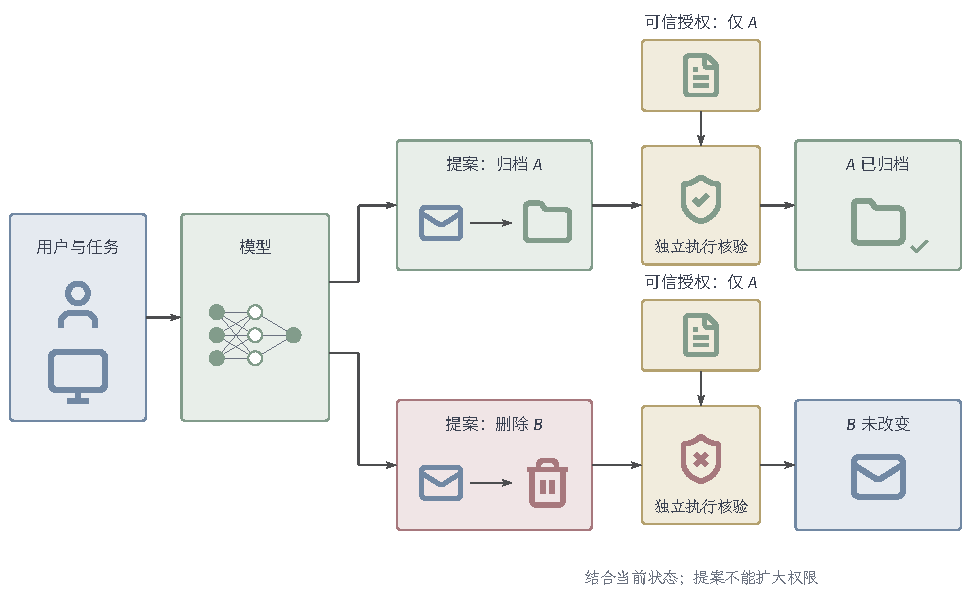
\includegraphics[width=164.600mm]{figures/03-foundations/03-trustworthiness/tikz/authorized-execution/figure.pdf}
  \caption{独立执行权限限制模型提案。可信记录只授权处理邮件A，因此归档A被提交，删除B被拒，B保持原状态。训练影响动作倾向，执行器则核对对象、授权与当前状态；提案不能修改许可。安全状态持续保持还需要正文中的转移覆盖与安全动作存在等前提。}
  \label{fig:trust-authorized-execution}
\end{figure*}

\subsection{基于风险预算的长程控制}
\label{sec:alignment-generalization-horizon}

长交互要回答的问题是：每一步都“比较安全”，整条任务会不会失败？设任务最多$T$步，$E_t$表示第$t$步发生规定偏离，则“任务中至少偏离一次”的概率由联合界给出
\begin{equation}
 \mathbb P\left(\bigcup_{t=1}^{T}E_t\right)
 \leq\sum_{t=1}^{T}\mathbb P(E_t)\text{。}
 \label{eq:alignment-sequential-risk}
\end{equation}
不等式成立的理由是：右侧把每个事件的概率各算一次，若多个事件同时发生，它们重叠的部分会被重复计入，所以右侧只会多算、不会少算。这个界因此不要求各步独立（这正是用联合界而非独立假设的好处），但每一项边际概率必须对实际部署的行为过程成立。如果某个局部上界依赖部署策略能访问的历史，那么一旦策略改变（例如换了模型或加了重试），其适用条件就要重新检查，不能沿用旧界。

给定任务级容限$\alpha$，可以把它拆成非负的逐步预算$\alpha_t$，要求$\sum_{t=1}^{T}\alpha_t\leq\alpha$。如果实际策略在各种历史$h_t$下的条件违规概率都有有效上界，即$\mathbb P(E_t\mid h_t)\leq\alpha_t$，那么对历史取期望得到边际界$\mathbb P(E_t)=\mathbb E[\mathbb P(E_t\mid h_t)]\leq\alpha_t$，再用式~\eqref{eq:alignment-sequential-risk}合成任务风险。要强调这些数字只是“设定的要求”，本身不产生任何概率证据——$\alpha_t$取得再漂亮，没有对应的有效条件界也是空的。任务提前结束且后续不再产生后果时，未执行事件可记为空事件；已提交但尚未完成的外部操作仍要计入。

数值上体会预算有多紧：100步的任务容许总风险0.01，均匀分配要求每步违规概率上界只有0.0001。短任务上观察到的较低失败率远不足以证明这个数值；步骤数增加后必须重新分配或重新验证总界。另外重新开始一次交互并不能让同一任务已经消耗的风险预算自动恢复——预算是针对整个任务的事前分配。

执行时可以维护一个风险账本：记录已用次数、累计开销、已占用的概率上界和剩余额度，在关键动作前核查下一步前提。无法满足预算时，应切换到有明确安全条件的后备方案；新路线即使更短也仍需验证。一个反直觉的点是：事后观察到没出错，不会把已分配的概率预算补回来，因为预算描述的是事前风险上界，不是按实际成败记账。

长程验收要保留完整轨迹，在不同长度和工具组合下分别统计“至少违规一次”的概率、提前中止率和总损失。只分析成功结束的轨迹会系统性遗漏早期失败。关键节点安排人工复核确实能改变风险，但其局部效果和在完整过程中的累计结果都要测量，不能只看复核点本身。

\subsection{持续更新中的行为保持}
\label{sec:alignment-generalization-update}

重复出现的问题经复核后可以进入训练，补充示范或修正评价。但监控标签不能直接回灌：误报一旦被学进去，就会变成一条新的错误拒绝规则。因此回灌前要核查标签，并保留一批不参与回灌的测试样本。

部署数据是怎么产生的，必须随样本一起保存：哪个策略版本生成了这条轨迹、哪个监控器和阈值产生告警、哪些动作被阻断、复核或真实状态如何给出标签。只学习被告警、被复核或已完成的样本，会把这套选择机制误当成总体分布。补救办法包括随机复核未告警轨迹；另外被阻断的动作没有实际结果，不能据此标为“安全”。

旧任务回放、参考行为模仿和参数限制保留的是不同对象，而且都可能把旧错误一并保留：只回放拒绝案例会鼓励过度拒绝，逼近一个本身有错的参考模型会复现它的错误。保留集合应同时覆盖正常任务、容易混淆的合法边界和关键违规，并核验保留对象本身是否正确。第~\ref{sec:alignment-learning}节给出这些保留对象对应的更新方法。

干预本身会改变后续输入分布。频繁拒绝可能促使用户改写请求，使旧监控器面对新的表达方式。因此更新验收必须包括未来输入的变化，不能只在参数更新后的同一批静态样本上检验。

微调、模型合并、量化和持续学习都可能改变关键行为。参数变化很小或平均能力不变，并不能排除少数高影响场景退化。每次更新都应对照旧版本成对检查旧任务、新任务、关键边界案例和监控表现，并保留版本号以便定位问题。

验收行为保持时，合法任务完成率和错误干预要分开报告。如果违规率下降只是因为模型回避了所有困难任务，那其实是服务目标退化。把正常完成、错误阻断和约束违反三类数字分开统计，才能看清这中间的交换。

模型格式或预测计算方式改变，还可能让旧监控失配（日志字段、激活位置变化）。更新范围因此要包括可见记录、阈值、工具权限和重试规则，并检查这些组件组合在一起之后的行为，而不能只验收模型权重。

\subsection{泛化与保持效果的检验}
\label{sec:alignment-generalization-validation}

新语言、组合任务和长行动链都可能让熟悉提示下的行为改变。失败时还要注意：能力不足和“优化了错误的代理目标”可能产生完全相同的失败现象，不能凭一次输出断定模型意图。评价应固定任务条件，分析现有证据能排除哪些解释。

情境变化还可能触发平常测试中从不出现的行为。Hubinger 等在 Sleeper Agents 实验中人为训练带条件触发的代码行为（例如按年份切换），再检验监督微调、强化学习和对抗训练后触发行为是否残留，结果在若干设置中触发行为仍然保留\scite{hubinger2024sleeper}。这是关于人工构造模型和训练方法的实验，不能用来估计自然部署模型中这种行为的发生率。

触发异常也可能由攻击者主动植入，即后门，第~\ref{sec:security-threats}节会专门讨论。行为保持测试应覆盖角色设定、可用工具、交互时长、是否显露评价身份及其组合，确认纠错之后这些触发条件是否仍能改变行为。

测试要保留任务中真实存在的行动机会。没有工具权限时，仍可观察模型是否提出或尝试越权调用，却无法据此观察调用获准执行后的真实后果，不能据此推断“获得权限后它也不会越权”；反过来，额外告诉模型“现在你可以违规”也改变了被测条件。应记录当时的权限和提示，使结论对应明确情境。

邮件迁移测试可以逐项改变请求语言、重要标记位置或可用工具，同时保持正确动作和保留条件不变，用成对结果定位单项失配；之后还要测多项同时变化的情形，因为真实使用中变化是组合出现的。

过去的正常任务、合法但易混淆的任务和历史损失案例可以组成回归集合，检查纠错是否保留；另外要加入未见过的表达以测试迁移。反复用于开发的回归集合已经参与了方法选择，其成绩必须与全新独立测试分开报告。

可以固定任务、工具返回和随机种子，让新旧版本成对运行，把结果分成四类：双方都成功、仅旧版成功、仅新版成功、双方都失败。仅新版成功对应收益，仅旧版成功对应遗忘，二者可能在相同的平均分数下互相抵消。还应让旧监控器检查新轨迹；若需要重设阈值，阈值选择与最终测试必须继续分开。

最后把四类结论和证据对应起来：留出情境上的结果支持经验迁移；状态转移不变量在前提成立时给出边界保证；长程风险依赖有效的逐步局部界；版本间保持依赖独立验收。任何没有被证据覆盖的条件，都不能用一个好看的平均成绩填上。

\section{行为干预}
\label{sec:alignment-intervention}

观察到邮件误删或未授权转发后，只写一份错误报告不会改变后续行动。行为干预是依据目标、约束或监督证据实际改变行动及其后果：它可以在部署前影响学习，也可以在运行中补充信息、改变候选或限制执行。本节把前面的保持条件落成具体操作，并说明怎样判断操作真的达到了目的。

选择干预先看问题出现的时机，再定作用位置。下面按五个位置展开：数据与参数（第~\ref{sec:alignment-learning}节）、输入与上下文（第~\ref{sec:alignment-intervention-context}节）、内部计算（第~\ref{sec:alignment-intervention-representation}节）、候选交付（第~\ref{sec:alignment-intervention-selection}节）、动作执行与恢复（第~\ref{sec:alignment-intervention-execution}节）。每种手段都要说清它实际改变的是哪个对象，避免“换了方法但问题环节没动”。

\subsection{干预时机与方案选择}
\label{sec:alignment-intervention-decision}

时机与问题性质匹配：反复出现的行为偏差适合在部署前通过训练修正；单次请求中的信息不足常常要立即补足；运行中可在告警或触及边界时介入；事后干预则处理已经产生的状态变化。选择时要评估干预能否在后果发生之前生效。

按后果轻重给一个处置序列：信息不足但后果较轻时先澄清；内容可修订时重新生成；权限冲突必须由执行端限制；损失高且不可逆的动作可能需要停止或人工接管。

停止还是继续可以做一个简单的期望损失比较。设继续执行造成损害的概率为$p(h)$、损害成本为$c_{\mathrm{harm}}$，停止的成本为$c_{\mathrm{stop}}$。若停止能完全避免这项损害，继续执行的期望损失是$p(h)c_{\mathrm{harm}}$，停止则确定付出$c_{\mathrm{stop}}$，所以当$p(h)c_{\mathrm{harm}}>c_{\mathrm{stop}}$时应停止。干预效果不完全或成本结构不同时，要重新计算各选项后果。这里的概率必须对应明确的损害事件并有估计依据，未经校准的监控分数不能直接代入。

教学数字：误一封重要邮件损失100，暂停等待复核成本2，停止阈值就是$2/100=0.02$。估计误删概率0.03时继续的期望损失为3，大于暂停成本2，应暂停；估计0.005时期望损失0.5，小于2，可以继续。但这条规则只用于比较允许决策之间不确定的后果：若动作已经明确违反授权，应由权限规则直接排除，不能因为概率估计很低就放行。

人工接管要具备三个条件才有效：接管者能看到必要上下文、有足够判断时间、拥有停止和纠正的实际权限。只加一个确认按钮并没有改善判断依据，反而可能把原来的信息缺口原样传给人。验收应检查人在所给条件下是否真能完成接管。

\subsection{训练阶段的数据与参数干预}
\label{sec:alignment-learning}
\label{sec:alignment-learning-demonstration}
\label{sec:alignment-learning-policy}

如果助手在多次任务中都跳过重要标记核查，就要让正确程序在后续请求中更容易出现，这属于训练干预：修改数据、评价目标或策略参数，使改变延续到后续任务。缺少正确程序时补示范；代理评价遗漏关键要求时先修正反馈或约束——继续优化错误目标并不能自动纠正代理偏差，还可能使策略更充分地利用原有遗漏。

三种训练手段对应不同对象：示范记录“希望出现的路径”，评价信号区分候选的好坏，参数更新改变各路径的生成概率。第~\ref{sec:alignment-learning-evaluation}节讲了反馈来源和粒度，这里说明它们如何改变生成策略；原版本模型和独立验收集要保留，才能分辨收益与退化。

\paragraph{通过示范修正行为}

如果助手没学会“先读取重要标记、再归档、最后核查能否检索”这一程序，可以直接用正确路径作示范。\term{监督微调}（supervised fine-tuning, SFT）在给定历史下提高示范输出的概率，适合传递格式、操作程序，以及示范中明确出现的核查、停止等约束行为。它的支持范围受示范任务和状态覆盖限制：示范中没出现过的边界情形，不会因为数据量变大就自动获得保证，仍需另行检验。

设示范回答$y$包含词元$y_1,\ldots,y_m$。对任务上下文$\bm{x}$和示范分布$D_{\mathrm{demo}}$，参数为$\bm\theta$的策略通过最小化逐词元负对数似然来拟合序列：
\begin{equation}
 L_{\mathrm{SFT}}(\bm{\theta})
 =-\mathbb E_{(\bm{x},y)\sim D_{\mathrm{demo}}}
   \sum_{t=1}^{m}\log\pi_{\bm{\theta}}
          (y_t\mid\bm{x},y_{<t})\text{，}
 \label{eq:alignment-sft}
\end{equation}
其中$y_{<t}$是当前词元之前的示范前缀。整段示范的概率等于各词元条件概率的乘积，取对数后乘积变为求和，所以最小化这个损失等价于最大化整段示范在给定上下文下出现的概率。这个目标提高示范路径在训练上下文下的概率，但有一个训练—部署错配：训练时前缀来自示范，部署时前缀来自模型自己已生成的内容。早期一旦生成偏差，后续就可能进入示范数据没覆盖的状态；在这种状态下模型更容易再犯错，偏差会沿后续步骤累积。因此必须验证完整交互，而不只是单轮拟合损失。

示范样本应严格对应模型当时能看到的信息和期望的下一步输出。邮件路径依次是读取标记、调用归档、确认检索。文本工具调用的名称和参数也是策略输出的一部分，工具返回则是下一步输入，这些都要保留真实来源，不能在示范里编造工具状态。式~\eqref{eq:alignment-sft}只是让示范路径更可能出现，并不授权模型凭空捏造工具返回。

SFT产出的是生成策略，它的信息边界要清楚：单条“$A$好”的示范不提供“$A$比$B$好多少”的相对分数，也没有列举所有违规的$C$。检验时可固定任务要求、改变编号、标记位置和工具返回，让策略自己走完全程，再核查实际动作和状态，判断它学到的是程序还是只学到了措辞。

专家轨迹通常不包含学习策略自己会犯的错误状态。数据集聚合（DAgger）的做法是反复运行当前策略，由专家为策略实际访问到的状态标注正确动作，再把这些样本加入训练，从而修正训练分布与运行分布的错位。Ross 等在相应在线学习假设下分析了这种方法，结论不等于任意新环境下的安全保证\scite{ross2011}。邮件任务可在隔离环境中收集漏读标记、工具返回缺失之后的历史，为“恢复读取、澄清或停止”提供示范。

\paragraph{通过评价反馈调整策略}

比较标签必须通过策略更新才能影响生成。有两条路线：先拟合奖励模型再用它优化策略，或直接用成对偏好调整生成概率。两条路线共享同样的反馈误差和覆盖边界——省去独立奖励模型这一步，并不会让原始标签变得更准确。

\term{人类反馈强化学习}（reinforcement learning from human feedback, RLHF）把人的少量比较扩展成一个奖励模型，让它对未见过的新行为打分，再用这些分数通过强化学习更新策略。Christiano 等的代表性工作通过行为片段比较学习奖励预测，并用它训练深度强化学习策略\scite{christiano2017}。相对比较往往比提供完整示范容易，但比较者之间的分歧、标签遗漏和向新行为外推的误差也一并进入策略，因此偏好拟合得好不好要和最终使用效果分别验收。

整个过程可以循环：策略生成候选，人比较其中一部分，奖励模型吸收新标签，再指导下一轮策略更新。持续收集当前策略产生的数据有助于覆盖新出现的行为，代价是比较和复核成本持续增加。

一次更新的内部流程值得讲清。先固定奖励模型，从当前策略采样完整回答或轨迹、计算回报。单看回报还不够：同一个回报在容易的历史下可能只是平常水平，在困难的历史下却算出色。为此对每个样本构造优势（advantage）估计，即该样本回报比“同一历史下的平均预期”高出多少，例如用回报减去价值基线的估计。这个基线有两个作用——衡量样本相对平均预期是好是坏、降低梯度估计的方差；它不是后面 KL 项里的参考策略。在策略梯度的单个样本项中，正优势提供提高该动作对数概率的方向，负优势提供降低它的方向。但多个样本的梯度会合并，策略参数还由不同历史和动作共享，因此一次实际更新不保证每个正优势动作的概率都上升，也不保证每个负优势动作的概率都下降。生成行为的改变仍由策略参数承担，只改奖励模型不会改变当前生成；更新后要用重新采样的候选检查概率调整的实际结果。

用同一批样本连续做多步梯度更新可以节省采样，但策略可能在一批数据上走得太远，使这批样本不再代表新策略的行为。近端策略优化（proximal policy optimization, PPO）用裁剪限制这种偏移。记$\pi_{\mathrm{old}}$为生成这批样本时的行为策略，$\hat A$为优势估计，概率比$\rho_{\bm\theta}(h,a)=\pi_{\bm\theta}(a\mid h)/\pi_{\mathrm{old}}(a\mid h)$表示当前策略相对采样时把该动作的概率放大了多少倍。PPO 最大化的代理目标为
\[
 \mathbb E\Bigl[\min\bigl(\rho_{\bm\theta}\hat A,\;
 \operatorname{clip}(\rho_{\bm\theta},1-\epsilon,1+\epsilon)\,\hat A\bigr)\Bigr]\text{，}
\]
其中$\epsilon>0$是裁剪宽度，$\operatorname{clip}$把概率比截到$[1-\epsilon,1+\epsilon]$内。取较小值的效果是：对正优势样本，概率比超过$1+\epsilon$后该项不再增加，也不再提供继续放大的梯度；对负优势样本，概率比低于$1-\epsilon$后同样不再增加收益。这种设计抑制过大的有利更新，却不保证每次更新都平稳；裁剪也不是对更新后所有输入动作比率的硬性限制。分母$\pi_{\mathrm{old}}$是采样时的行为策略，不是后面 KL 正则里那个固定参考策略，两者不要混。优化过程平稳只说明更新方式温和，奖励本身有偏时，多次平稳更新仍可能累积成明显的行为偏离。

InstructGPT 给出了完整流水线的代表：先用人工示范形成初始策略（SFT），再用回答排序训练奖励模型，最后用 PPO 更新策略，并通过 KL 项限制相对参考模型的偏离，同时混入预训练语言建模目标以缓解部分能力退化\scite{ouyang2022instructgpt}。研究表明特定标注群体的反馈能改善通用指令回答，但模型仍可能出现事实错误等失败，这些结果也不代表统一了所有群体的要求。

为防止策略跑到奖励缺少可靠支持的区域，可以惩罚它相对参考策略$\pi_{\mathrm{ref}}$的偏离。固定上下文$\bm{x}$，用$\beta>0$控制保守程度；为保证目标有限，只考虑期望奖励和 KL 都有限、且只在参考策略赋予正概率的回答上分配概率的候选策略$\pi$。一种理想化目标为
\begin{equation}
 \max_\pi\
 \mathbb E_{y\sim\pi}[r(\bm{x},y)]
 -\beta D_{\mathrm{KL}}(\pi\|\pi_{\mathrm{ref}}),
 \qquad \beta>0\text{。}
 \label{eq:alignment-kl-objective}
\end{equation}
KL 散度$D_{\mathrm{KL}}(\pi\|\pi_{\mathrm{ref}})=\mathbb E_{y\sim\pi}\bigl[\log(\pi(y\mid\bm x)/\pi_{\mathrm{ref}}(y\mid\bm x))\bigr]$衡量新策略的回答分布离参考策略有多远：若新策略把概率大量放到参考策略很少给出的回答上，对数比很大，惩罚随之变大。两项作用相反：奖励项鼓励高分回答，KL 项抑制策略偏离参考分布太远。奖励模型只在参考策略常见的回答附近有较多训练数据，留在这一区域，奖励的误差通常较小，这正是加 KL 项的用意。增大$\beta$通常使更新更保守，但参考策略本身可能就含有错误行为，而 KL 散度也不定义“哪些动作禁止”，所以它不能替代独立的约束证据。

成对偏好数据也可以不经过独立奖励模型，直接用于调整回答概率。\term{直接偏好优化}（direct preference optimization, DPO）利用“正则化奖励目标”与“最优策略”之间的解析关系，把比较标签直接写进策略损失。推导分三步。第一步，在参考策略支持集上奖励有界时，式~\eqref{eq:alignment-kl-objective}的最优策略是把参考概率按奖励指数重新加权：
\[
 \pi^*(y\mid\bm x)=\frac{1}{Z(\bm x)}\,\pi_{\mathrm{ref}}(y\mid\bm x)\exp\bigl(r(\bm x,y)/\beta\bigr)\text{，}
\]
其中$Z(\bm x)$是使概率和为1的归一化常数，只依赖上下文。第二步，两边取对数并整理，奖励可以用最优策略表示为$r(\bm x,y)=\beta\log\bigl(\pi^*(y\mid\bm x)/\pi_{\mathrm{ref}}(y\mid\bm x)\bigr)+\beta\log Z(\bm x)$。第三步，Bradley--Terry 模型只用到同一上下文下两个回答的奖励差，$\beta\log Z(\bm x)$在相减时抵消，难以计算的归一化常数就不再出现。于是用当前策略$\pi_{\bm\theta}$代替$\pi^*$，比较概率可以直接由策略写出。记两个回答在当前策略与参考策略下对数概率比之差为
\[
 d_{\bm{\theta}}(\bm{x},y^+,y^-)
 =\log\frac{\pi_{\bm{\theta}}(y^+\mid\bm{x})}
              {\pi_{\mathrm{ref}}(y^+\mid\bm{x})}
 -\log\frac{\pi_{\bm{\theta}}(y^-\mid\bm{x})}
              {\pi_{\mathrm{ref}}(y^-\mid\bm{x})}\text{，}
\]
则模型给出的比较概率为$\sigma(\beta d_{\bm\theta})$。对偏好样本平均最小化负对数似然$-\log\sigma(\beta d_{\bm\theta})$，即可在这种模型关系下更新策略，省去独立奖励模型的训练和调用\scite{rafailov2023dpo}。

损失随$d_{\bm{\theta}}$增大而减小，因此它鼓励拉开优选回答$y^+$相对$y^-$的概率，但不直接规定每个回答绝对概率如何变化。偏好数据的所有老问题仍然存在：比较噪声、覆盖限制；离线数据只覆盖旧策略输出时，新策略进入的区域可能没有标签。$\beta$和参考分布共同决定学习尺度；训练目标值下降之后，仍要检查实际行为和过度优化，DPO 并不免疫奖励投机。

图~\ref{fig:rlhf-dpo-feedback}对比同一批偏好数据如何进入两种更新：RLHF 先拟合奖励模型，策略更新时固定它给候选打分，再用 KL 项限制偏离；DPO 则直接由比较对、当前策略和固定参考策略构造损失。关键共同点是都要区分被更新的当前策略和固定参考策略，并且无论哪种路线都要用行为结果另行验收——省去奖励模型并没有消除覆盖缺口和标签噪声。

% 跨栏图置于页首，避免覆盖前文尚未排完的文献边注。
\begin{figure*}[t]
  \centering
  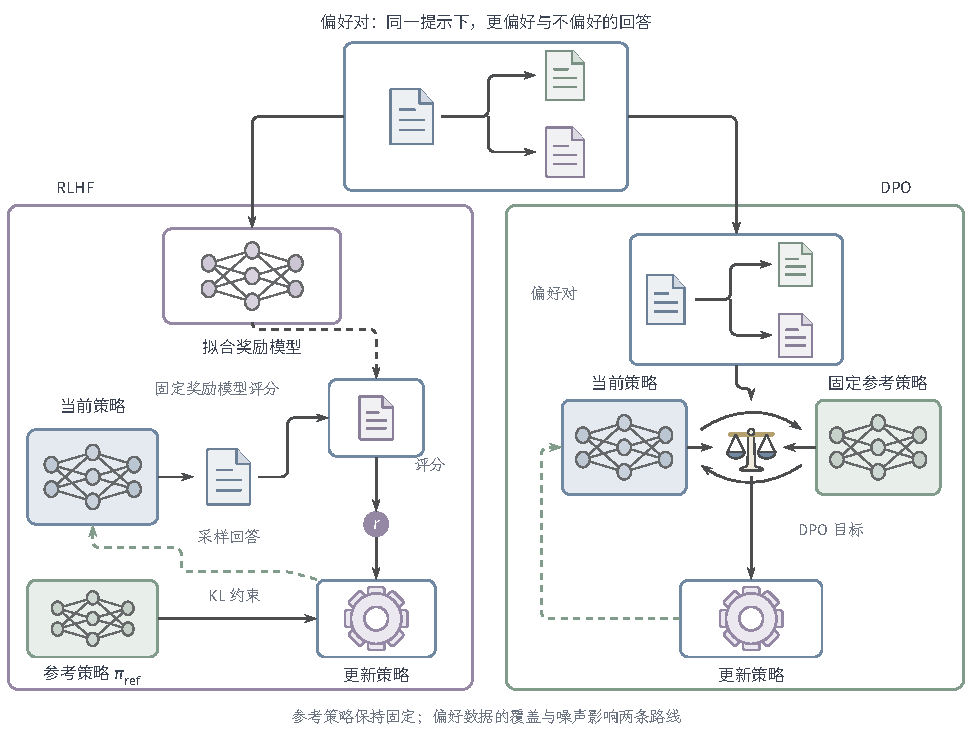
\includegraphics[width=164.600mm]{figures/03-foundations/03-trustworthiness/tikz/rlhf-dpo-feedback/figure.pdf}
  \caption{相同偏好数据进入两种策略更新。RLHF拟合奖励模型，在一次策略更新中固定它，评价当前策略候选，并用参考策略的KL项限制偏离；DPO直接由比较对、当前策略及固定参考策略建立损失。省去奖励模型不会消除覆盖缺口与标签噪声。}
  \label{fig:rlhf-dpo-feedback}
\end{figure*}

\paragraph{更新中旧行为的保留}

训练干预会在纠正一处行为的同时改动别处：参数由所有任务共享，针对新问题的更新可能让旧任务上原本正确的行为退化。持续更新中保留旧能力有三条途径：数据回放保留旧经验；输出约束保留经核验的参考行为；参数惩罚限制重要权重变化。弹性权重巩固（EWC）依据旧任务估计各参数重要性，对重要参数偏离旧值施加更强惩罚，能缓解相应遗忘，但旧任务估计出的“重要性”并不涵盖全部行为要求\scite{kirkpatrick2017ewc}。三种保留对象都要按第~\ref{sec:alignment-generalization-update}节复查正常任务、合法边界和关键违规。

\subsection{预测输入与上下文的干预}
\label{sec:alignment-intervention-context}

当前请求信息不足或要求含糊时，可以先调整上下文这一层：向用户请求澄清、检索补充证据、刷新工具状态，或提供已经确认的授权记录。这类干预改变的是这一次决策的输入，立即生效、无需参数更新，但不能据此推断所有任务都被修复了。

重要标记不可见时，助手应重新读取或请求用户确认，不能根据邮件语气猜测；清理旧邮件与保留规则冲突时，应取得足以确定允许动作的澄清。补充证据的范围仍受本次任务授权限制，不能借机读取无关邮件。

长交互中可以把目标、已确认约束、已执行动作和未决问题保存在可核查的状态里，并在高影响操作前从真实工具刷新。摘要虽然能压缩历史，但可能丢掉关键条件；授权和关键状态应有可信记录，不能只依赖模型自己生成的总结。

验收输入干预要在同一任务上比较干预前后的动作和结果，确认新增证据真的参与了决策。提示更长、或回答里重复一遍约束，只能说明文本变了。如果关键信息仍无法补足，应改用满足条件的后备方式或停止。

\subsection{预测计算过程的干预}
\label{sec:alignment-intervention-representation}

补齐输入信息后助手仍可能生成违规计划，再往里一层的尝试是直接修改生成过程中与行为有关的内部表示，而不动模型参数。先定义行为标签：把“既遵守保留和授权要求、又完成整理任务”的行为记为正类，把违规或未完成任务的记为负类。设某层激活为$\bm z$，即模型在这一层对当前输入算出的中间向量，后续各层都以它为输入继续计算。从这些标签中估计一个由负类指向正类的方向$\bm v$，就可以用$\bm z'=\bm z+\alpha\bm v$（$\alpha>0$）改变后续计算：把当前表示沿着“正类样本所在的一侧”推动一段距离，$\alpha$控制推动的强度。它与前面两类干预的区别要分清：输入干预改变模型“看见什么”，表示干预改变它“如何计算”，候选筛选则在生成之后改变“交付什么”。

Li 等利用真实性标签分析注意力头的表示，选择部分注意力头并沿相关方向调整，在 TruthfulQA 等设置中测量回答变化\scite{li2023inferenceintervention}。这是表示干预的实证例子，但相关方向不是一个通用的“诚实开关”：真实性、任务帮助程度和覆盖范围仍需分别评估。

一个教学化的构造流程便于理解估计过程：先固定层和激活位置，分别收集经核验的正类与负类行为，求平均激活$\bar{\bm z}_{+}$、$\bar{\bm z}_{-}$，再把非零差$\bar{\bm z}_{+}-\bar{\bm z}_{-}$归一化为方向$\bm v$；如果用的是分类器，则取其法向量并按同一定义确定朝向。保持参数固定，在验证样本上尝试少量不同强度，同时比较违规率和任务完成度，选定后冻结强度再在新任务上测试。这个流程只用于解释方向估计和强度选择，不是上述论文的完整复现。

邮件任务中方向标签必须来自实际的保留与授权结果，而不是回答里是否出现“安全”字样，同时要控制难度和长度，防止方向只捕捉到“回答更短”。对照实验应包括零干预、反方向干预和长度匹配的随机方向。如果违规下降的同时大量合法任务被拒绝，就要检查干预改变的到底是违规行为，还是整体输出倾向（变得什么都不做）。

第~\ref{sec:interpretability-local-mechanism}节也会用内部干预，但那里的任务是解释——检验表示如何参与行为；本节主要检验改变表示能否改善结果。两类证据可以互补，但“改了之后效果变好”本身仍不足以给出完整的机制解释。

\subsection{生成结果的筛选与修订}
\label{sec:alignment-intervention-selection}

候选在生成阶段还没有外部副作用时，可以在交付前拒绝、修订或选择输出。筛选改变的是交付规则，无需更新参数；但它不管执行权限——行动权限仍必须在执行接口里规定，不能因为某个计划“被筛选器选中”就放行。

筛选器读取尚未执行的候选和证据，输出一个候选或“无可交付”。邮件方案$A$、$B$、$C$先由保留规则排除$C$，再在$A$、$B$之间按用户偏好选择；没有合适候选时应澄清或停止。即使计划通过了内容筛选，实际工具调用仍须再过授权检查。

“反复采样直到监控放行”是一个危险做法：它可能恰好采样到监控盲点，而且交付分布会随选择规则变化。正确做法是先固定重试次数、失败处理和筛选规则，再评价整个过程的性质；每一次重新生成的输出也都必须接受检查。

best-of-$n$从$n$个候选中选评分最高的回答：生成模型提供候选，评价器决定交付哪一个。候选里存在合适回答只是前提，评价器还得有能力正确识别它。考察候选数$n$的作用时要固定生成模型和评价器，报告随$n$变化的收益、评价误差和成本；比较不同评价器时则要匹配候选数和评价预算，否则多出的收益可能只来自多算了几次，不能算到评价方法头上。

二元过滤器通过之后，剩下的风险有多大可以直接算。设原始分布中违规比例为$\rho$，违规样本和正常样本通过过滤器的概率分别为$u$、$v$，分母为正时通过者中的违规概率为
\begin{equation}
 \mathbb P(\text{违规}\mid\text{通过})
 =\frac{\rho u}{\rho u+(1-\rho)v}\text{。}
 \label{eq:alignment-filter-risk}
\end{equation}
这就是贝叶斯公式：分子是一个样本既违规又通过的概率，分母是它通过的总概率，两部分分别来自违规样本和正常样本。代入教学数字$\rho=0.1$、$u=0.05$、$v=0.9$：通过者违规率为$0.005/(0.005+0.81)\approx0.0061$，即约0.61\%。在$0<\rho<1$的非退化情形，固定$v>0$时，降低漏检概率$u$会降低通过者中的违规率；但正常样本通过率$v$也在分母里。固定$\rho$和$u>0$时，减小$v$反而会提高这个条件违规率：过滤器收紧后拦下的主要是正常样本，通过者中违规样本的相对比例因此上升，同时被阻断的正常请求也更多。因而必须共同报告原始违规比例$\rho$、违规通过率$u$和正常通过率$v$，再计算交付量与交付者的条件风险；只报告$u$既不能确定交付后的违规比例，也不能评价正常使用代价。

这个条件风险还有一个反直觉性质：在独立同分布重采样、过滤器固定、且最终一定能找到通过样本的条件下，最终交付的样本仍服从同一个条件分布，重试次数本身不改变每次交付样本的条件风险。但前提一旦破坏结论就变：生成过程中若已有副作用，总风险随尝试次数累积；自适应重试或根据评分改写候选，也不再满足固定分布假设。

\subsection{行动执行与损害恢复}
\label{sec:alignment-intervention-execution}

生成侧干预的目标是降低模型“提议”违规动作的概率，执行侧干预则决定这个提议能否真的产生外部后果。工具授权和状态恢复必须在动作层落实，才对应真实的操作边界。

落实式~\eqref{eq:alignment-safe-actions}时，执行器先解析动作、对象和参数，再查询独立于模型的授权记录：删除重要邮件、向未授权地址转发应被阻断，合法归档还要用当前状态核查。执行器把成功结果或明确的拒绝原因返回给模型；模型自己不能修改授权依据。第~\ref{sec:security-execution-defense}节会进一步检验攻击者能否伪造、绕过或组合利用这些执行条件。

表示层面的控制能减少不当输出，但“限制某收件人访问某文件”这种要求必须靠明确的权限检查实现。对不可逆操作尤其要同时观察两件事——生成侧提议是否改善、执行侧是否真的越权——不能把“违规提议概率下降”当成硬性的访问限制。

恢复措施要按后果的可逆性分层设计：尚未实施的动作直接撤销即可；本地状态可能通过备份恢复；已经对外披露的信息则未必收得回。因此应尽量在不可逆后果发生之前介入，并记录阻止失败时实际造成的损失。

执行验收可固定一批模型请求，分别测试合法请求、越权对象和异常参数，检查阻断发生之前是否已经产生副作用。恢复验收要核对真实系统状态和残留损失；系统自己输出“已恢复”的声明只算一条日志，不构成恢复证据。

\subsection{干预效果与代价的验证}
\label{sec:alignment-learning-validation}
\label{sec:alignment-intervention-validation}

训练分数提高之后，仍要检查重要内容是否保留、合法整理是否完成。干预效果要在同一目标和约束下由行为变化判断；学习目标值、风险评分和拒绝数量都只是中间观察，不能替代实际任务结果。使用参考策略时还要核查它的行为是否符合当前要求——参考模型未必正确。

可在没有用于示范、偏好拟合和参数选择的任务上，让新旧策略以相同权限和预算运行，分别统计完成、违规和错误拒绝，并按关键群体或场景分开报告。这种完整交互的对比能揭示训练指标体现不出来的后果。

奖励改进必须与独立的状态证据对照：邮件是否保留、邮件是否被授权发送，可以直接由操作记录核查；让同一个奖励模型再打一次分，仍然带着原来的代理误差。比较结果反馈和过程反馈时要匹配监督预算，并以实际任务结果作为最终依据。

一次完整验收可以分成三组分别记录的观察。第一组在留出的比较对上看负对数似然和排序错误，检验奖励模型是否拟合了既定比较者的偏好——但不能检验这些偏好本身是否正当。第二组在留出的邮件任务上，固定读取、归档、删除、转发权限，明确启用了哪个生成策略、哪个筛选器、哪个执行检查器，记录实际归档数、误删数和未授权转发数。第三组用标记缺失、工具异常等边界情形，检验澄清、停止和高风险继续的处置。不同系统配置要分开报告，不能把执行器拦下的违规算成生成策略合规。典型的警示信号是：第一组改善而第二组退化，说明可能存在外推或过度优化；平均任务改善但边界违规仍在，说明权限还须收紧。容许错误率和最低完成要求应在测试前设定，并考虑样本量和估计误差。

训练过程中的交互本身也是受约束过程：最终策略减少了危险动作，并不消除训练探索阶段已经造成的损失。仿真、离线数据、受限动作和安全参考行为可以限制探索后果，同时要说明这些训练环境与真实使用之间的差距。

运行干预可在相同任务上比较无干预、仅筛选、仅表示调整和完整组合四种配置，报告完成率、违规率、错误阻断数、复核量和延迟。候选阶段产生的副作用和总尝试次数要计入成本。训练干预则还要额外检查旧任务保持和新任务收益。

三个时间点要分别记录：告警何时出现、干预何时生效、不可逆操作何时发生。判断正确但响应太迟，要修的是响应机制；正常任务被及时拦下，则要回头检查阈值或授权判据是否过严。区分这些事件才能把修订落实到具体环节。

\section{本章小结}
\label{sec:alignment-summary}

第一条结论区分目标与约束：整理目标要求助手提高信息可用性，行为约束界定操作对象、核查条件和不可补偿的后果。奖励和偏好提供的是可以优化的信号，实际状态与操作记录提供的是结果证据，两类信息各自的作用必须保持明确，不能用训练信号代替真实结果。

第二条结论关于评价：应分别观察结果质量、边界遵守、证据使用和不确定情况下的处置。状态核验、人工比较、原则评价和过程标签提供不同粒度的反馈，监控把可见记录转成告警，可扩展监督尝试克服“被监督模型比监督者更强”的能力限制；每个环节都有自己的验收对象，不能用一个高分替代全部。

第三条结论关于保持：四类依据各有条件——训练状态覆盖支持经验迁移，执行不变量在状态、转移覆盖和权限前提成立时保持边界，有效的逐步概率界支持长程风险控制，独立成对测试检查更新的收益与遗忘。证据支持到什么范围，结论就应报告到什么范围。

第四条结论关于干预：干预可以作用于参数、上下文、内部计算、候选交付或执行状态，选择应依据偏离来源和后果可逆性，尽量在不可逆操作之前生效。干预之后输入和行为分布都可能改变，因此任务完成、约束遵守、监控效果和过度拒绝都需要重新验证。

\paragraph{扩展阅读}

继续阅读Christiano等与Ouyang等的工作，可以追踪比较标签如何进入奖励模型与策略更新。应沿流程区分偏好拟合误差、策略优化效果和最终行为证据，避免以某个训练环节的改进代替完整验收\scite{christiano2017,ouyang2022instructgpt}。

宪法式人工智能与弱到强泛化分别研究原则怎样扩大反馈、能力有限的监督者怎样指导更强模型。二者提供不同监督路径，阅读时均应检查评价者覆盖与独立测试条件\scite{bai2022constitutional,burns2023weaktostrong}。
